\chapter{一种新的神经网络压缩方法}

\section{背景}
现代神经网络由多种类型的层组成,输入在这些层中不断被传递和处理,从而被分类或识别。在每一层中,每一个神经元接收多个输入进行处理,并将输出通过突触送到下一层。目前主流的神经网络包括卷积神经网络神经网络 (CNNs) ,深度神经网络 (DNNs) 和循环神经网络(RNNs)。目前深层神经网络已经在图像识别, 目标检测,语音识别,自然语言处理,视频处理领域有了越来越广泛的应用。虽然这些神经网络非常强大,但是大规模的神经网络参数(包括神经元和权值)对存储和带宽提出了很高的需求,例如,AlexNet的网络规模超过$200MB$,VGG-16的网络规模超过$500MB$,这使得这些大规模的深度神经网络难以在嵌入式设备,特别是移动设备上进行部署。

首先,对于百度和Facebook等公司,手机端的各种应用程序更新都是通过不同的应用程序商店进行下载,它们是对二进制文件的大小非常敏感。例如,应用程序商店会限制当应用程序大于$200MB$时,必须连接无线网络才能够进行下载。因此,当应用超过$200MB$时,将会收到比$10MB$应用更多的安全审查。尽管在手机端本地运行深度神经网络能够减少网络带宽,进行任务实时处理,获得更好的隐私保护,但是这些大规模的神经网络需要耗费巨大的存储开销,因此阻碍了深度神经网络应用被部署到移动应用程序。

第二个问题是能耗问题。大型神经网络需要大量的带宽加载神经网络数据(包括拓扑结构,输入,神经元,权值等),同时需要大量的计算资源完成神经网络的运算,这个过程需要耗费巨大的能量。考虑到移动设备电池容量的限制,高能耗的应用,如深层神经网络应用将难以部署。能源消耗主要来源于访存能耗。在$45nm$工艺下,一个32位浮点加法需要消耗$0.9pJ$的能量,一次32位SRAM缓存访问耗费$5pJ$的能量,而一次32位DRAM内存访问需要$640pJ$的能量,这个能耗几乎是浮点加法操作的3个数量级。大型神经网络无法缓存在片上的SRAM中,因此需要需要在片外的DRAM与片上的SRAM之间频繁进行数据交换,从而产生巨大的访存能耗开销。例如我们以$20fps$运行一个拥有10亿个连接的神经网络,那么需要为DRAM访存提供至少$P = (20Hz)\times (640pJ)\times (1G) = 12.8W$的功率,这个已经完全超过了大多数手机电池能够提供的功率。

\subsection{神经网络中的稀疏特性}
虽然现代神经网络在许多应用中占主导地位,但是庞大的参数给计算、内存容量和内存访问带来了沉重的负担。为了应对这些挑战,研究者从各个方向做出了各种各样的努力,包括算法级 (例如Drop out~\cite{srivastava2014dropout}、Sparsity~\cite{han2015learning}),架构级 (例如短位宽运算~\cite{holi1993finite}甚至是1比特运算~\cite{rastegari2016xnor}、非精确计算~\cite{venkataramani2014axnn})和物理级(例如,动态电压调整技术~\cite{pillai2001real})。其中,稀疏技术是目前解决这个问题最有效的方法。研究人员在早期工作中已经证明了稀疏性是解决过拟合问题的有效方法。对于现代神经网络,研究者们提出了一系列的训练技术,如稀疏编码 (Sparse Encoder)~\cite{olshausen1996emergence},自动编解器 (Auto Encoder/Decoder)~\cite{boureau2008sparse,lee2008sparse}, 深度信念网络 (Deep Belief Network, DBN)~\cite{lee2007efficient}等,在不影响精度的前提下修剪冗余的突触和神经元。最近,研究人员提出了一种新的剪枝方法~\cite{han2015learning},在CNNs上获得了非常理想的稀疏性,在AlexNet~\cite{krizhevsky2012imagenet}网络上获得了$88.85\%$的稀疏度, 在VGG16~\cite{simonyan2014very}网络上获得了$92.39\%$的稀疏度。在表~\ref{tab:deepratio},我们报告详细的剪枝结果,这里,我们定义稀疏度 (sparsity) 为被修剪的神经元/突触占总神经元/突触的比例,同时我们定义稠密度(density)为非零神经元/突触占总神经元/突触的比例。


\begin{figure}[h]
  \centering
  \begin{minipage}[t]{\columnwidth}
  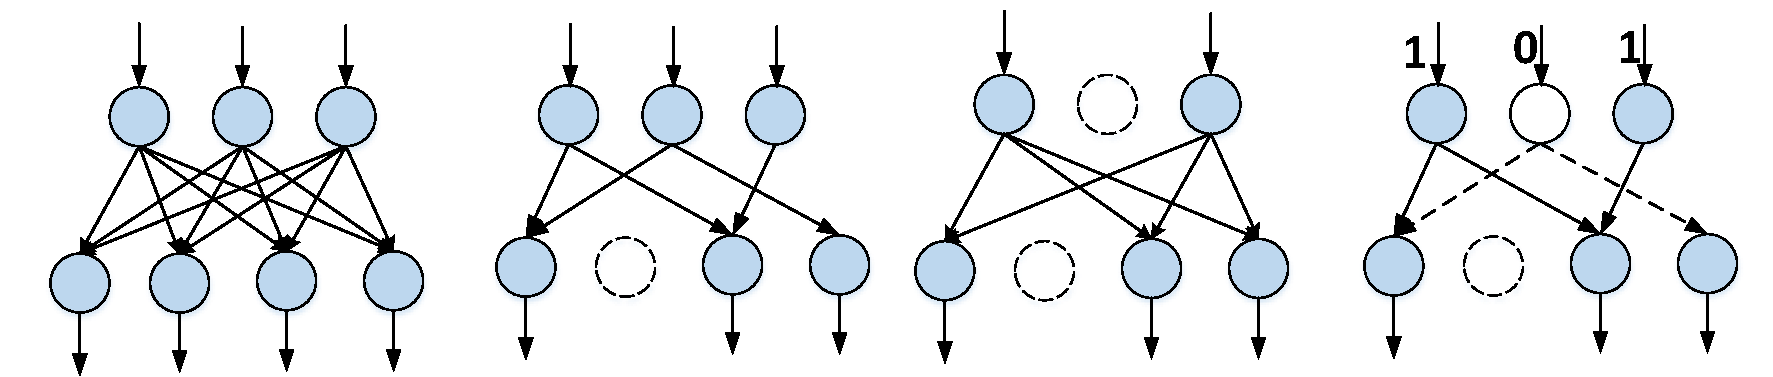
\includegraphics[width=1.0\columnwidth]{sparse_network.pdf}
  \end{minipage}
  \vfill
  \begin{minipage}[t]{0.24\columnwidth}
      \centering\footnotesize
    (a)
  \end{minipage}
  \hfill
  \begin{minipage}[t]{0.24\columnwidth}
      \centering\footnotesize
    (b)
  \end{minipage}
  \hfill
  \begin{minipage}[t]{0.24\columnwidth}
      \centering\footnotesize
    (c)
  \end{minipage}
    \hfill
  \begin{minipage}[t]{0.24\columnwidth}
      \centering\footnotesize
    (d)
  \end{minipage}
  \caption{ (a) 稠密神经网络 (b) 静态权值稀疏 (c) 静态神经元稀疏 (d) 动态神经元稀疏}
  \label{fig:sparsity}
\end{figure}

如图~\ref{fig:sparsity}所示,我们将神经网络中的稀疏分为两类:\emph{静态稀疏 (static sparsity)}和\emph{动态稀疏 (dynamic sparsity)}。\emph{静态稀疏}源于剪枝操作,当突触 (图~\ref{fig:sparsity} (b)) 或者神经元 (图~\ref{fig:sparsity} (c)) 满足某些条件时,它们将从神经网络的拓扑结构中被永久剪除,那么在预测(inference)过程中,网络的拓扑结构并不会随着输入的变化而发生改变,即稀疏神经元或者稀疏权值的位置不随着输入而发生改变,因此这种稀疏又被称为\emph{静态稀疏}。当神经元的激活值为$0$时(图~\ref{fig:sparsity} (d))会发生\emph{动态稀疏}, 特别是当使用ReLU作为激活函数时,在ReLU激活之前结果为负的神经元输出值为$0$。形式上,ReLU用如下公式计算输出神经元
\begin{equation}
ReLU(x)=
\begin{cases}
x & \text{if } x > 0, \\
0 & \text{if } x \leq 0
\end{cases}
\end{equation}
其中$x$为ReLU激活函数的输入,$yR$为ReLU的输出。因此,像ReLU这样的激活函数可以在网络的神经中中引入许多$0$。不同于~\emph{静态稀疏},\emph{动态稀疏}不改变网络拓扑结构,它与输入密切相关,因为不同的输入将导致不同的计算结果,从而导致不同的动态稀疏结果。值得注意的是,\emph{静态稀疏}又可以分为\emph{静态权值稀疏 (static synapse sparsity, SSS)}和~\emph{静态神经元稀疏 (static neuron sparstiy, SNS)},\emph{动态稀疏}仅由\emph{动态神经元稀疏 (dynamic neuron sparsity, DNS)}组成。

\subsection{权值编码}

\begin{figure}[h]
\centering
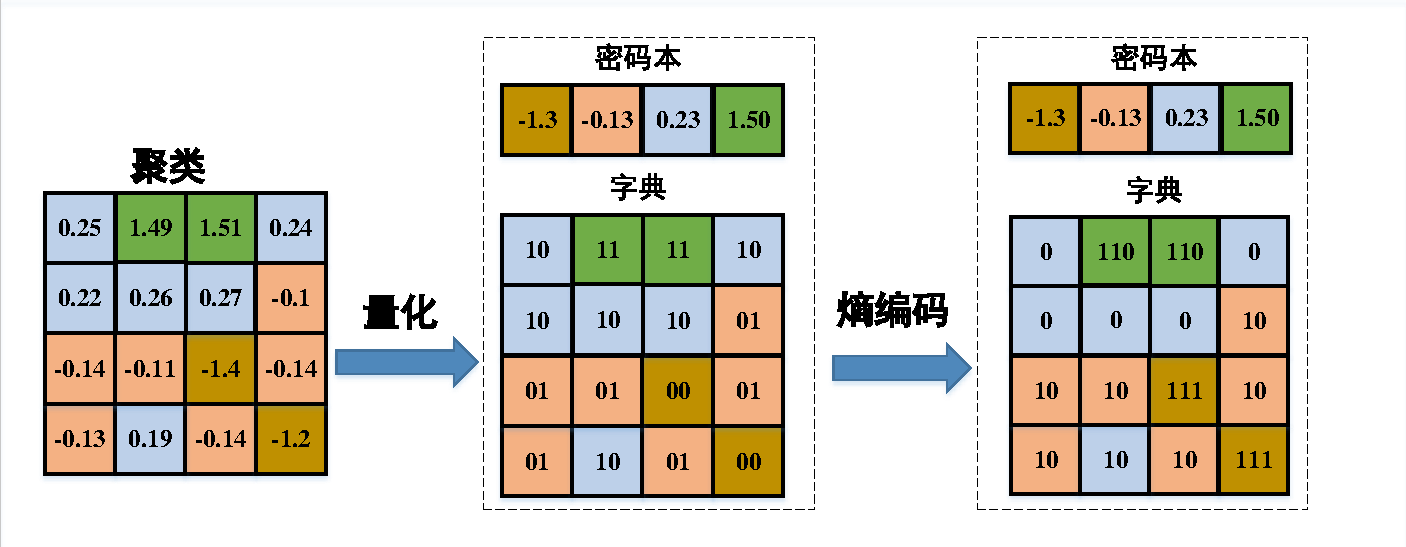
\includegraphics[width=1.0\columnwidth]{WE.pdf}
\caption{权值编码过程}
\label{fig:weight_encoding}
\end{figure}

为了进一步压缩权值数据,研究人员将图像压缩技术,如量化 (quantization)~\cite{henneaux1992quantization},熵编码 (entropy coding)~\cite{mackay2003information}等应用到神经网络的领域。Deep Compression~\cite{han2015deep}运用细粒度剪枝,全局量化和霍夫曼编码对神经网络进行深度压缩,在基本不损失精度的情况下,在AlexNet网络上获得35倍的压缩比,在VGG网络上获得了49倍的压缩比。另一种有效的压缩方案是CNNpack~\cite{wang2016cnnpack},它在频域中对神经网络进行深度压缩,最终在AlexNet网络上获得了40倍的压缩比,在VGG网络上获得了46倍的加速比。我们在图~\ref{fig:weight_encoding}中描述了权值编码的过程,它由量化和熵编码两个步骤组成。

\subsubsection{量化}
量化的定义

首先,我们利用聚类算法 (例如,K-means聚类算法~\cite{}) 将分散的权值聚集成$K$个簇,其中值相近的权重将会被聚成一个簇。在图中,16个权值被分为4个簇,其中 (0.25, 0.24, 0.22, 0.26, 0.27, 0.19)这六个权值被聚为一个簇,(-0.1, -0.14, -0.11, -0.14, -0.13, -0.14)这六个权值被聚为一个簇,(1.49, 1.51)这两个权值被聚为一个簇,(-1.4, -1.2)这两个权值被聚为一个簇。每一个簇对应一个中心值,该值与簇中所有权重的总距离最小,同一个簇中的所有权值都用它所在簇的中心值来近似表示,例如在图中,(0.25, 0.24, 0.22, 0.26, 0.27, 0.19)这六个权值聚成的簇的中心点为0.23,因此我们用0.23近似表示这六个权值;同理,我们用-0.13近似表示(-0.1, -0.14, -0.11, -0.14, -0.13, -0.14)这六个权值;用1.50近似表示(1.49, 1.51)这两个权值;用-1.3近似表示(-1.4, -1.2)这两个权值。因此,我们可以用一个密码本和一个字典来表示所有权值,其中密码本中记录了$K$个簇中的中心值以及每个中心值的索引,例如图例中的密码本((00, -1.3), (01, 0.13), (10, 0.23), (11, 1.50))。字典中每个元素只需要$log(K)$位的索引来表示,我们可以通过索引密码本从而获得权值。

\subsubsection{熵编码}

\begin{figure}[h]
\centering
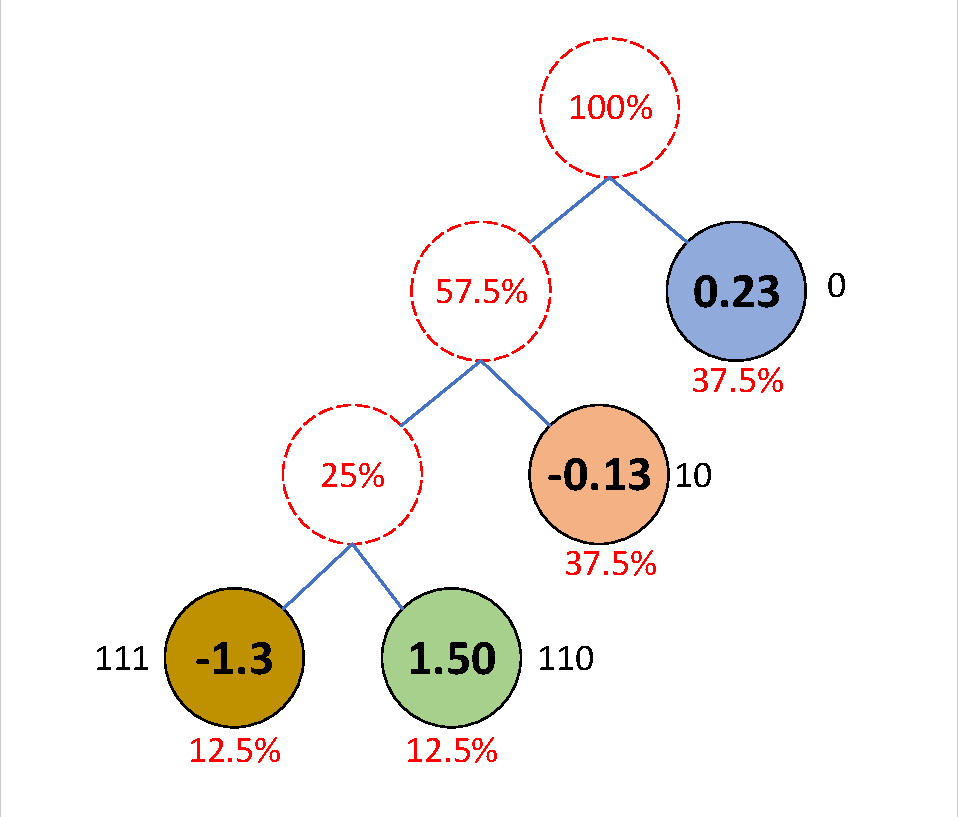
\includegraphics[width=0.6\columnwidth]{huffman.pdf}
\caption{哈弗曼树}
\label{fig:huffman}
\end{figure}

熵编码即编码过程中按熵原理不丢失任何信息的编码,因此它是一种无损压缩的编码技术。熵解码是熵编码的逆过程,能够完整地解码出原始码流中的信息,常见的熵编码有:香农编码(Shannon coding),哈夫曼编码(Huffman coding)~\cite{huffman1952method}和算术编码(arithmetic coding)~\cite{witten1987arithmetic}。
信息熵为信源的平均信息量(不确定性的度量),具体来说,符号$\alpha_i$所表示的信息熵为
\begin{equation}
I(\alpha _i) = -\log p(\alpha _i)
\end{equation}

信息流$Y$的包含的信息熵$H(Y)$为
\begin{equation}
H(Y) = -sum_{i=0}^{m-1} p(\alpha _i) \log p(\alpha _i)
\end{equation}

由于密码本中元素的出现概率是不平衡的,因此我们可以采用熵编码(如哈弗曼编码)进一步降低表示权重的比特数。哈弗曼编码方法完全依赖于码元出现的概率来构造整体平均长度最短的编码方法。进行哈夫曼编码的关键步骤是建立符合哈夫曼编码规则的二叉树,该树又称作哈夫曼树。哈夫曼树是一种特殊的二叉树,其终端节点的个数与待编码的码元的个数等同,而且每个终端节点上都带有各自的权值。每个终端节点的路径长度乘以该节点的权值的总和称为整个二叉树的加权路径长度。在满足条件的各种二叉树中,该路径长度最短的二叉树即为哈夫曼树。在使用哈夫曼编码执行对码元的实际编码过程时,通过递归地合并概率最小的码元来构建哈夫曼树。以图~\ref{fig:weight_encoding}为例,四个码元-1.3,-0.13,0.23,1.50出现的概率分别是0.125,0.375,0.375,0.125,最终可以构造出如图~\ref{fig:huffman}所示的哈弗曼树。在哈夫曼树构建完成后,便可以得到每一个码元的哈夫曼编码的码字。具体方法是:从哈夫曼树的根节点开始遍历,直至每一个终端节点,当访问某个节点的左子树时赋予码字1,访问右子树时赋予一个码字0(反之亦然),直到遍历到终端节点时这一路径所代表的0和1的串便是该码元的哈夫曼编码码字。例如,在图中,最终四个码元-1.3, -0.13, 0.23, 1.50分别被编码成为是111,10,0,110。

\subsection{不规则性}
尽管稀疏神经网络能够在理论上减少计算量,存储量和数据传输量,但是稀疏会导致原本规则的神经网络计算模式转变为不规则的形式。然而,目前的处理平台由于存在诸多问题,无法有效地处理稀疏性。根据~\cite{zhang2016cambricon},CPU和GPU并不能很好地支持稀疏神经网络运算,即使使用稀疏矩阵运算库,如sparseBLAS或者cuBLAS,也不能取得非常理想的加速效果,在某些情况下处理稀疏网络的性能甚至比处理稠密神经网络的性能还要差。例如,CPU平台上,除了 LeNet-5 网络,稀疏的AlexNet网络和VGG16网络的性能都比稠密网络channel,性能平均降低了2.11 倍。在GPU平台上,运行稀疏神经网络仅仅能提高$23.34\%$的性能,对比于稀疏神经网络高达$90.84\%$的稀疏度,这个性能提升是非常有限的。因此通用的CPU和GPU并不能利用稀疏的特性。尽管目前又不少支持稀疏神经网络的加速器~\cite{zhang2016cambricon, albericio2016cnvlutin, han2016eie, han2017ese, angshuman2017scnn},但是它们仍然不能有效地处理稀疏神经网络带来的不规则性。他们需要显著的稀疏成本,而且不能完全支持所有稀疏类型,例如Cambricon-X~\cite{zhang2016cambricon}中支持稀疏的逻辑占总面积的$31.07\%$,占功耗的$34.83\%$,而且只能支持权值稀疏。Cnvlutin~\cite{albericio2016cnvlutin}只能利用神经元稀疏。EIE~\cite{han2016eie}虽然能够同时利用权值和神经元稀疏,但是它只能适用于稀疏的全连接层,不能运行稀疏卷积层。SCNN~\cite{angshuman2017scnn}能够在卷积层同时利用神经元和权值稀疏,但是对全连接层的支持并不理想。因此,我们需要一种新的神经网络稀疏方法,能够在保持高的精度和稀疏度条件下尽可能保持神经网络的规则性,减少稀疏神经网络的不规则性,有利于CPU,GPU或者加速器能够充分利用稀疏带来的收益。


\section{局部收敛 (local convergence)}

\begin{figure}[h]
  \centering
  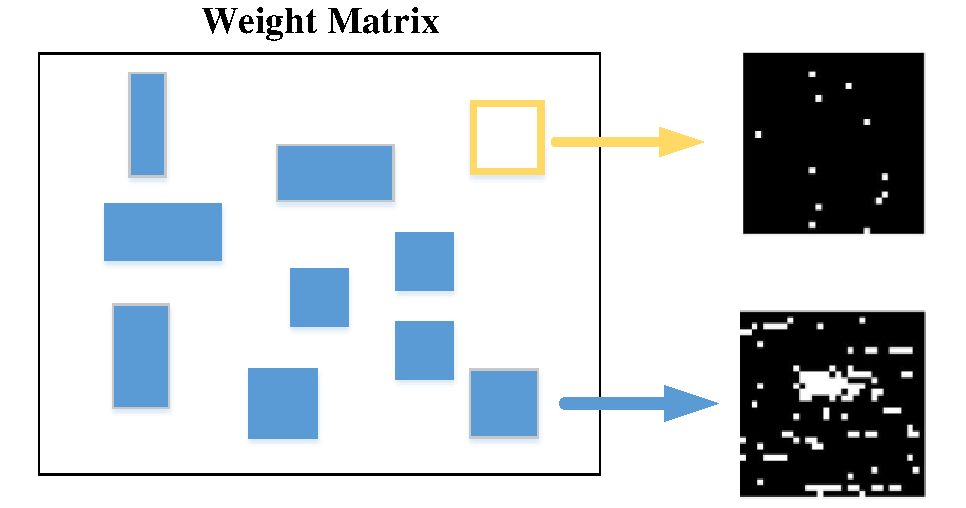
\includegraphics[width=0.8\columnwidth]{local_convergence.pdf}
  \caption{全连接层中的局部收敛现象(白点表示大权值,绝对值大于其余$90\%$的权值)}
  \label{fig:local_convergence}
\end{figure}

传统的剪枝方法将单个突触当作独立不相关的元素,当突触符合特定的剪枝条件时(如权值的绝对值小于某一个阈值),该突触将会被剪除,但是这种方式忽略了突触之间的潜在关系。我们充分分析了神经网络中的权重分布情况,观察到了一个有趣的现象。如图~\ref{fig:local_convergence}所示,我们使用权值矩阵来表示全连接层的权值,每一行包含与对应输入神经元相连接的所有权值,每一列包含与对应输出神经元相连接的所有权值;我们可以发现,绝对值大的权值往往会聚集成簇,我们将这种现象称为局部收敛(local convergence)。我们利用如下的方式证明局部收敛的存在。首先,我们在权值矩阵上设定一个大小为$k$的滑动窗口,然后将该滑动窗口沿着权值矩阵空间维度上进行滑动(全连接层权值矩阵为两个维度,卷积层权值矩阵为四个维度),同时统计窗口中较大权值的数量,如果某一个权值的绝对值大于剩余$m\%$的权值,我们将其定义为较大的权值。为了方便阐述,我们将一个具有$x$个大权值的窗口标记为$x$窗口。我们选择了5个代表性的层: AlexNet网络的~\emph{fc6}层, VGG16网络的~\emph{fc6}层, MLP网络的~\emph{ip1}层, LSTM网络的~\emph{$W_{ix}$}层, AlexNet网络的~\emph{conv2}作为驱动示例。我们将前四层网络的滑动窗口大小设为$k = 4$, \emph{conv2}层网络的滑动窗口大小设为$k = 2$,此外,我们将$m = 90$设置为较大权值的阈值。在图~\ref{fig:cdf}中,我们描绘了一个随机初始化层与训练后的5个层中较大权值的累计分布。我们观察到,在初始化层中,同一个窗口中较大权值的数量不会超过四个。但是,这五个训练过的层存在同一个窗口中较大权值的数量超过七个的情况。因此,较大权值在训练过程中趋向于聚集在一起,也就是局部收敛。

\begin{figure}[t]
\centering
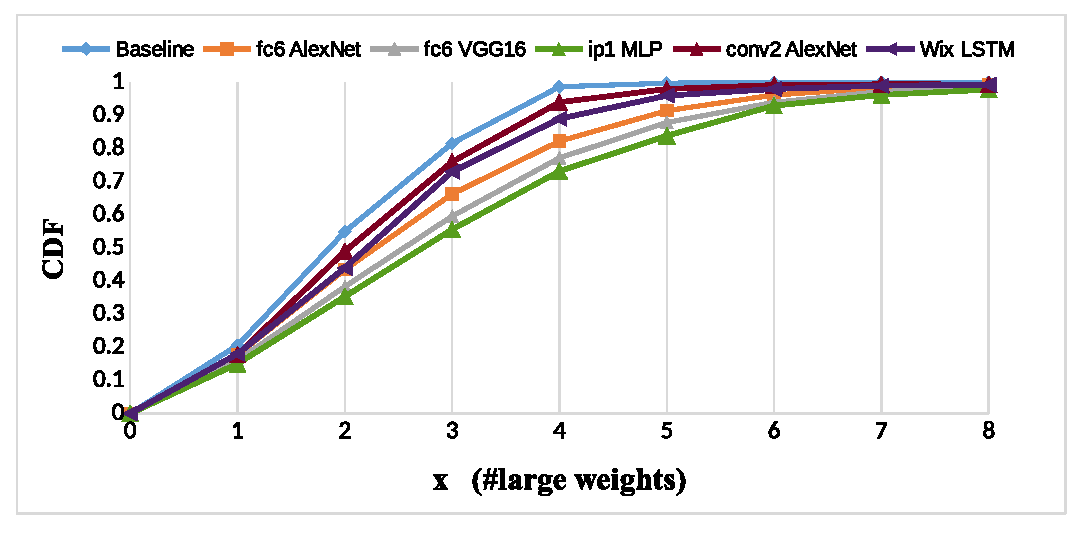
\includegraphics[width=0.8\columnwidth]{CDF.eps}
\caption{较大权值的累计分布}
\label{fig:cdf}
\end{figure}

\section{压缩神经网络}

\begin{figure}[h]
\centering
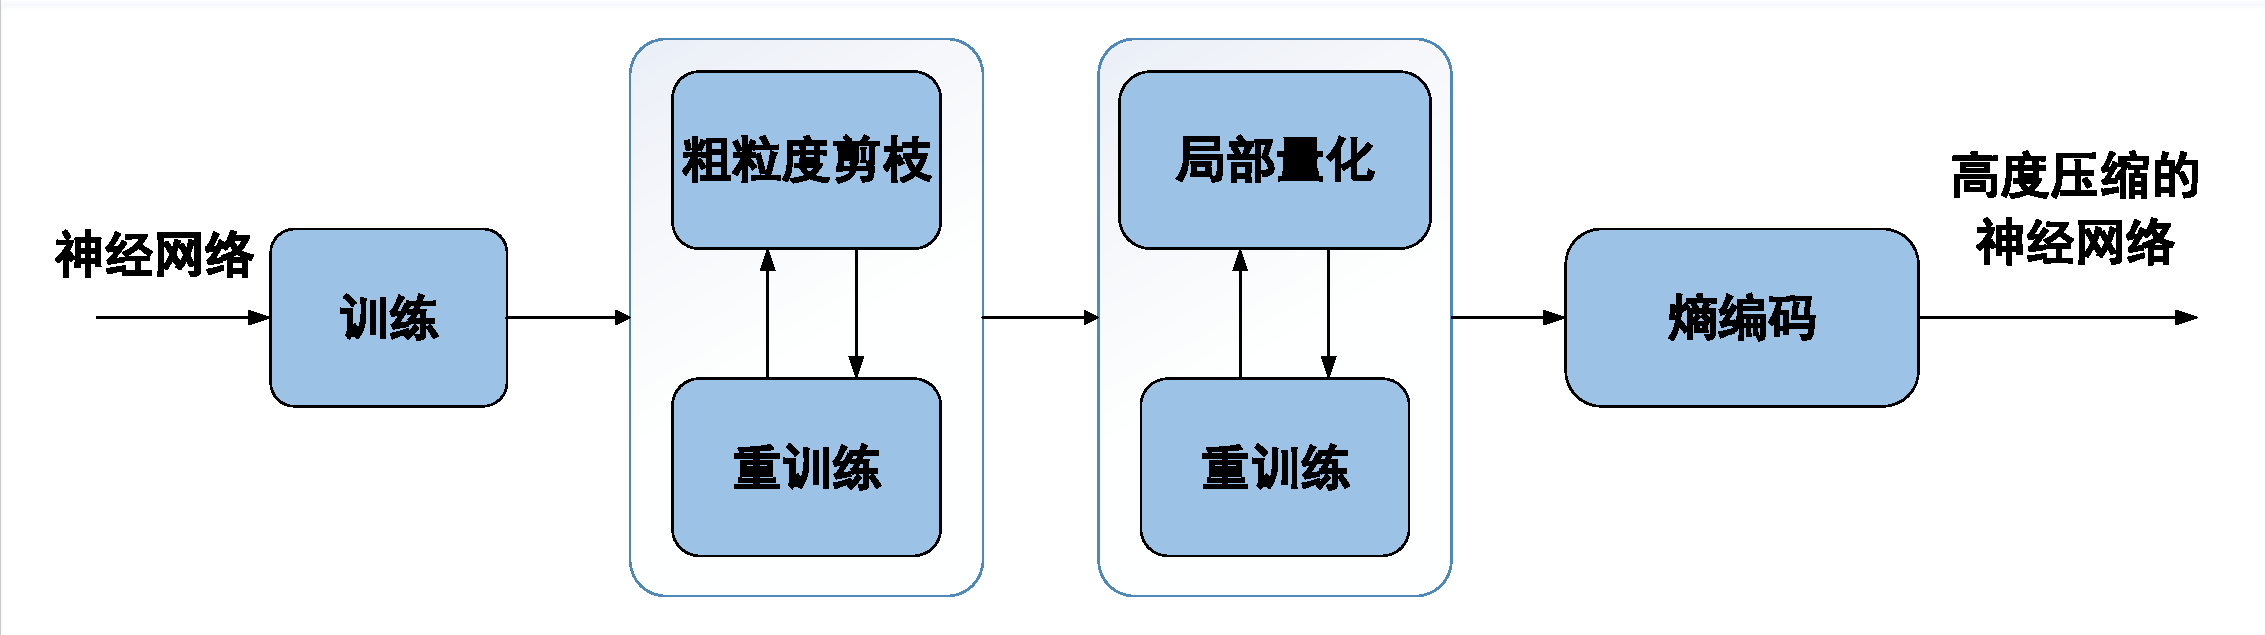
\includegraphics[width=1.0\columnwidth]{compression_flow.pdf}
\caption{新的压缩神经网络步骤}
\label{fig:compression_flow}
\end{figure}

如图~\ref{fig:compression_flow}所示,我们提出了一种新的压缩神经网络的方法,整个流程包括三个步骤:粗粒度剪枝,局部量化和熵编码。下面我们将依次详细阐述这三个步骤。


\subsection{粗粒度剪枝}

我们提出了一种新的剪枝策略:粗粒度剪枝。粗粒度剪枝的核心思想基于神经网络局部收敛的特征,我们将多个突触同时进行剪枝操作,而不是对单个权值进行剪枝。我们首先将权值矩阵分成多个块,如果某一个符合特定的条件,这个权值块将在网络拓扑中被永久剪除,然后我们使用较小的学习率对网络进行重训练,从而保持网络的准确性。值得注意的是,我们在训练中迭代地应用粗粒度剪枝和重训练,以获得更好的稀疏性,同时避免精度损失。为了清晰地解释粗粒度剪枝技术,我们使用全连接层~\ref{fig:fc_pruning}和卷积层~\ref{fig:conv_pruning}作为驱动示例。

\subsubsection{剪枝策略}

\begin{figure}[h]
\centering
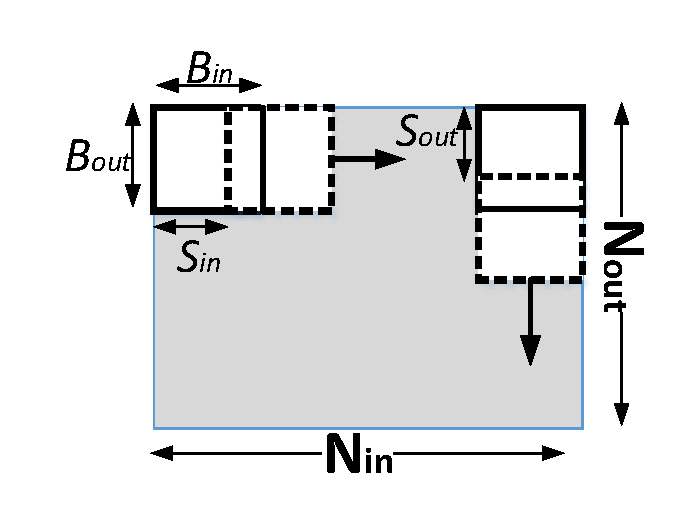
\includegraphics[width=0.7\columnwidth]{fc_pruning.pdf}
\caption{全连接层上的粗粒度剪枝}
\label{fig:fc_pruning}
\end{figure}

在一个全连接层中,($N_{out}$)个输出神经元通过二维权值矩阵($N_{out}$, $N_{in}$)与($N_{in}$)个输入神经元,如图6所示。在剪枝过程中,大小为$B_{in} \times B_{out}$的滑动窗口沿着权值矩阵的两个维度分别按照$S_{in}$和$_{out}$的步长进行滑动。一旦滑动窗口中的权值某些条件,窗口内的突触都会同时被剪枝。在迭代剪枝过程中,滑动窗口将跳过修剪过的突触,使所有修剪过的突触块都具有相同的规模大小,从而简化索引过程。

对于卷积层,输出特征图中的输出神经元通过共享的突触连接到输入特征图中的神经元。因此,卷积层中的权值可以表示为一个四维张量,即$(N_{fin},N_{fout},K_x,K_y)$,其中$N {fin}$是输入特征图的数量,$N {fout}$是输出特征图的数量,和$K x$,$K_y$是卷积核的大小。如图所示,在剪枝过程中,大小为$B_{fin} \times B_{fout} \times B_x \times B_y$的滑动窗口沿着四维的权值张量分别按照$S_{fin}$,$S_{fout}$,$S_x$和$S_y$的步长进行滑动。

\begin{figure}[h]
  \centering
  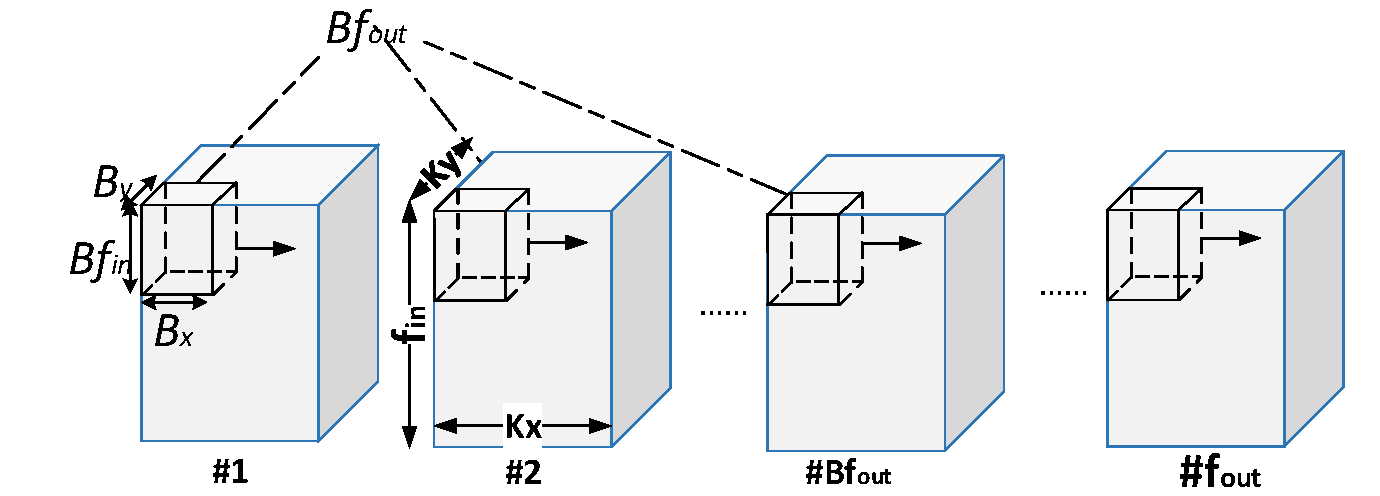
\includegraphics[width=1.0\columnwidth]{conv_pruning.pdf}
  \caption{卷积层上的粗粒度剪枝}
  \label{fig:conv_pruning}
\end{figure}

\subsubsection{剪枝块大小}

在粗粒度剪枝过程中,寻找最佳的剪枝块大小来权衡压缩比与精度之间的平衡至关重要。使用过大的块进行剪枝将导致突出连接无法完全表达神经网络的特性,从而降低准确性。使用过小的块进行剪枝,并不能充分利用局部权值收敛的特性,从而无法获得很高的压缩比。值得注意的是,如果我们将剪枝块的大小设定为1,那么粗粒度的剪枝就是~\cite{han2015learning}中的细粒度剪枝。

在本文中,我们仔细权衡神经网络中不同类型层的块大小来修剪不同的网络。理论上,我们应该为不同的层选择剪枝块大小,而不是为不同类型的层选择剪枝块大小,但是考虑到在庞大的设计空间搜索和极长训练时间,我们关注的是为网络中不同类型的层设定剪枝块大小。例如,由于卷积层中的权值比全连接层的权值更敏感,因此我们只在卷积层的某个维度上进行粗粒度剪枝。我们以AlexNet为作为驱动实例,在保持网络准确性的同时,阐述不同剪枝块的大小对神经网络稀疏度和压缩效果的影响。如表~\ref{tab:blocksize}所示,我们将AlexNet网络的基准精度设定为top-1误差$42.8\%$,同时我们使用$(1,N,1,1)$和$(N,N)$的剪枝块分别对卷积层和全连接层进行粗粒度剪枝。在表2中,我们将卷积层和全连接层的权值分别用8位和4位进行量化,然后用Huffman编码进行编码。当$N$从1增加到64时,压缩比$r_c$首先从40倍迅速增长到79倍,然后迅速下降到65倍。当剪枝块从1增大到16时,压缩比随之增加,主要原因是非零权值索引所需的存储空间不断减少。当剪枝块大小从16增加到64时,压缩比随之下降,这是因为为了保持相同的精度,神经网络的稀疏度不断降低(卷积层稀疏度从$64.75\%$降低到$54.45\%$),从而阻碍了压缩比。为了更好地平衡压缩比和精度,我们将卷积层中的剪枝块大小设置为$(1,16,1,1)$,将fc6,fc7和fc8的剪枝块大小分别设定为$(32,32)$,$(32,32)$和$(16,16)$。值得注意的是,使用粗粒度剪枝,非零权值索引所需要的存储空间只需要$29.38KB$,相比于使用细粒度剪枝后~\cite{han2015deep}的索引($2.95MB$)减少了102.82倍。

\begin{table}[b]
\centering
\caption{ 不同剪枝块大小情况下AlexNet网络的稀疏度和压缩比(C: 卷积层;F: 全连接层; S: 稀疏度; $r_c$ 压缩比)}
\label{tab:blocksize}
\begin{tabular}{lll@{~}llll@{~}llll@{~}llll@{~~}llll@{~~}llll@{~~}llll@{~~}lllllllll}
\toprule
N  				& 1 	&  2		& 4			& 8			& 16		& 32 		&64		\\
\midrule
C:S(\%)			& 64.99 &64.99		&64.89		&64.77		&64.75		&59.95		&54.45 	\\
F:S(\%) 		& 89.99	&89.98		&89.98		&89.97		&89.95		&89.91		&87.78	\\
Weight (MB)     & 2.86 	&2.86		&2.87		&2.87		&2.91		&3.01		&3.59	\\
Index (MB)      & 2.95	&0.76		&0.22		&0.07		&0.03		&0.01		&0.005	\\
$r_c$ 			& $40\times$ 	&$64\times$		&$75\times$		&$79\times$		&$79\times$		&$77\times$		&$65\times$	\\
\bottomrule
\end{tabular}
\end{table}

\subsubsection{最大值剪枝 vs. 平均值剪枝}

\begin{figure}[t]
  \centering
  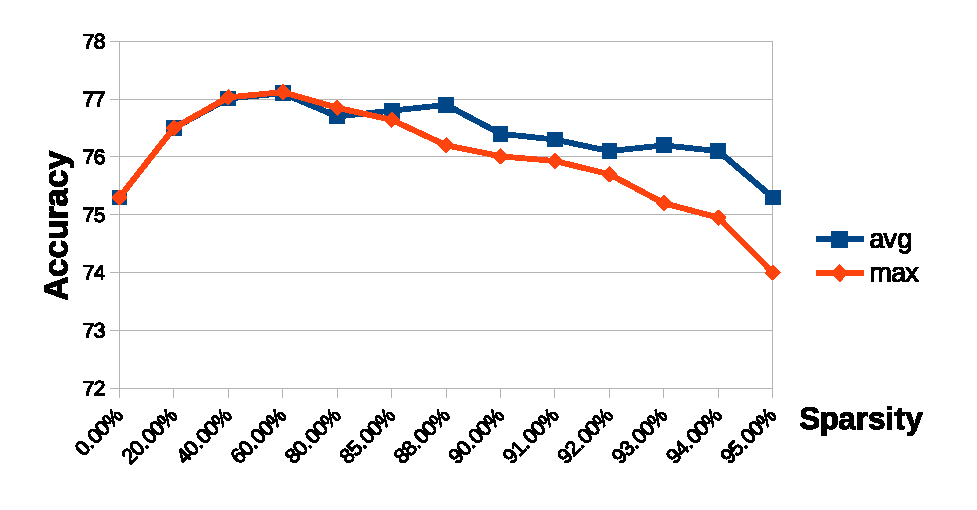
\includegraphics[width=1.0\columnwidth]{avg_max.eps}
  \caption{Cifar10快速模型上的最大值剪枝和平均值剪枝}
  \label{fig:max_or_avg_pruning}
\end{figure}

在粗粒度剪枝过程中,我们可以使用两种不同的剪枝策略,第一种是最大值剪枝策略,第二种是平均值剪枝策略。对于最大值剪枝策略,如果窗口中具有最大绝对值的权值小于预定义阈值($W_{th}$),则将窗口中的所有权值剪除。对于平均值剪枝,如果窗口中所有权值绝对值的平均值小于预定义的阈值,则将窗口中的所有权值剪除。这两种剪枝策略的主要特性是完全不同的。最大值剪枝表明只有块内部最大的权重才会影响整个块的重要性。平均值剪枝表明,块内的所有权重将对块的重要性产生影响。我们使用这两种剪枝方法在Cifar10快速模型上进行粗粒度剪枝和训练,在剪枝过程中我们控制这两种剪枝方法使用相同大小的滑动窗口和步长。图~\ref{fig:max_or_avg_pruning}显示,当神经网络的稀疏度高于$85\%$时,平均值剪枝比最大值剪枝精度更高。因此,本文选择了平均值剪枝的策略。

\subsubsection{不规则性的评估方法}
为了更直观地表现粗粒度剪枝的效果,我们提出了一种简单而有效的方法来定量测量粗粒度剪枝减少的不规则性。我们使用如下公式计算
\begin{equation}
R(Irr) = JBIG(I_f)/JBIG(I_c)
\end{equation}
其中$R(Irr)$表示减少的不规则性,$I_{f}$和$I {c}$分别表示经过细粒度剪枝和粗粒度剪枝后稀疏神经网络的索引,$JBIG()$表示基于Joint Bi-level Image ExpertsGroup~\cite{jbig}的无损二值图像压缩标准。这种方法基于这样一个事实:常规数据(特别是二进制矩阵)包含了更多的冗余信息,因此可以用更少的数据来表示。因此,我们将突触索引作为二进制图像,用JBIG压缩它们。压缩后的数据大小在某种程度上可以衡量数据的不规则性。因此,我们通过粗粒度剪枝与细粒度剪枝后压缩索引大小之比来度量降低的不规则性。

\subsubsection{神经元稀疏}
在粗粒度的剪枝过程中,我们只修剪突触,并不会对神经元进行直接修剪,仅仅当某个神经元与其他神经元之间没有任何连接时,该神经元会被剪除,因此静态神经元稀疏的比例并不高。然而,在大型网络中,动态神经元稀疏占了很大的比例,即神经元经过激励后的输出值为0的情况。在表x中显示了在各个网络中,权值稀疏性,静态神经元稀疏性和动态神经元稀疏性。在大规模神经网络中,如AlexNet、VGG16和ResNet-152,静态神经元稀疏性非常低,在卷积层中接近$0\%$,即基本不会出现静态神经元的情况。然而,在AlexNet和VGG16中,动态神经元稀疏性却很有前景,在AlexNet中为$37.63\%$,在VGG16为$59.48\%$,动态神经元稀疏为提高计算性能和节省能耗提供了很好的契机。

\begin{table}[b]
\centering
\caption{\footnotesize 神经网络中的稀疏性 (C: 卷积层; F:全连接层; SSS: 静态权值稀疏; SNS: 静态神经元稀疏; DNS: 动态神经元稀疏).}
\label{tab:sparsities}
\begin{tabular}{@{~}lll@{~}lll@{~}lll@{~}lll@{~}lll@{~}lll@{~}llllllllllll}
\toprule
-- & LeNet5 & MLP & Cifar10 & AlexNet & VGG16 & ResNet152 \\
%\hline
\midrule
C: SSS (\%)& 88.98 	& -- 	& 92.08 & 64.75 & 64.83 & 45.69 \\
   SNS (\%)& 25.39	& -- 	& 11.49 & 0.00 	& 0.00 	& 0.00 \\
   DNS (\%)& 0.00	& -- 	& 30.61 & 37.63	& 59.48 & 50.30 \\
\hline
F: SSS (\%)& 91.47	& 90.13	& 93.99 & 89.95	& 95.16 & 0 \\
   SNS (\%)& 47.70	& 40.25 & 57.73 & 15.75 & 22.18	& 0 \\
   DNS (\%)& 11.50	& 66.31 & 19.93	& 29.27 & 43.03	& 24.10 \\
\bottomrule
\end{tabular}
\end{table}

\subsection{局部量化}
\begin{figure}[h]
  \centering
  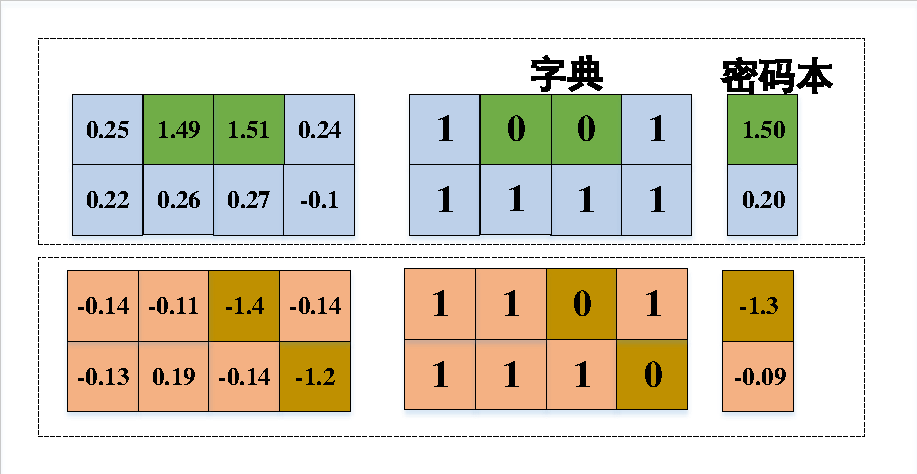
\includegraphics[width=1.0\columnwidth]{LQ.pdf}
  \caption{局部量化}
  \label{fig:local_quantization}
\end{figure}
应用权值共享和网络量化的策略可以有效地减少代表权值的比特位~\cite{han2015deep}。为了更好地利用局部收敛的特性,我们提出了局部量化的策略,不同于全局量化在整个权值矩阵中进行权值共享,局部量化仅仅在权值矩阵的局部区域中进行权值共享。如图~\ref{fig:local_quantization}所示,局部量化策略首先将权值矩阵划分为两个子矩阵,然后对两个子矩阵分别进行聚类。在每个子矩阵中,权值将被编码成一个密码本和一个字典,其中字典中的每个权值只需要1比特进行索引(使用图~\ref{fig:weight_encoding}中的全局量子化方法,密码本中每个权值需要2比特进行索引)。与全局量化相比,局部量化能够利用局部收敛来进一步减少表示权值的比特数,从而获得更高的压缩比。值得注意的是局部量化的开销很小,以AlexNet网络的fc6层为例,全局量化需要一个$128B$的密码本和$2.0MB$的字典,其中字典中每个元素需要5比特进行索引;局部量化过程中我们将权值矩阵分为64个小矩阵,因此需要64个密码本和64个对应的字典,但是字典中每个元素仅仅需要4比特进行索引,因此密码本和字典的大小分别为$4KB$和$1.6MB$,对比与全局量化存储容量减小了$19.81\%$。

\subsection{熵编码}
熵编码是一种无损的数据压缩策略,它为输入中的每个符号创建并分配唯一的无前缀码。由于每个码字的长度都与该符号出现概率的负对数成比例,所以我们使用更少的比特来编码出现概率更高的符号。目前两种最常见的熵编码技术是Huffman coding~\cite{huffman1952method}和算术编码~\cite{witten1987arithmetic}。实验显示,熵编码能够进一步减少$20\% - 30\%$的网络存储开销。

\subsection{压缩实验结果}
\begin{table}[h]
\centering
\caption{压缩后神经网络的稀疏度,压缩比和不规则性减少量 ($W_p$: 粗粒度剪枝后权值规模 ; $W_q$: 粗粒度剪枝,局部量化后权值规模; $W_c$: 粗粒度剪枝,局部量化,熵编码后权值规模; L: \emph{LSTM}层 ; C: 卷积层; F: 全连接层; W: 权值; I:权值索引;$r_p$: 粗粒度剪枝后压缩比; $r_q$: 粗粒度剪枝,局部量化后压缩比; $r_c$: 粗粒度剪枝,局部量化,熵编码后压缩比; $R(Irr)$: 不规则性减少量)。}
\label{tab:compression}
\begin{tabular}{@{}l@{~}l@{\!\!}l@{~}l@{\,}l@{~}l@{\,}l@{}l@{~}l@{~}l@{~}l@{~}lll}
\toprule
Model		&\!\!\!Sparsity(\%) & ~~$W_p(B)$ 	& $r_p$ 	& $W_q(B)$ 		& $r_q$ 		& $W_c(B)$ 		& $r_c$			& $R(Irr)$ 				\\
\midrule
Alexnet 	& C: 64.75\ 		&W: 25.65M  &$9\times$   &W: 3.60M 		& $64\times$ 	& W: 2.90M		& $79\times$	& $101.65\times$	 				\\
  			& F: 89.93\ 		&I: 36.73K  &  			 &I: 36.73K 	&  	 			& I: 29.38K 	& 				&		\\
%\hline
VGG16 		& C: 64.83\ 		&W: 42.72M  &$12\times$  &W: 7.80M		& $66\times$ 	& W: 5.25M 		& $98\times$	& $28.54\times$  	 				\\
  			& F: 95.16\  		&I: 202.80K &			 &I: 202.80K 	&  	  			& I: 121.68K	& 	  	 		&			\\
%\hline
LeNet-5 		& C: 88.98\ 		&W: 135.96K &$12\times$  &W: 23.77K 	& $66\times$  	& W: 19.01K		& $82\times$	& $8.87\times$ 	 				\\
  			& F: 91.47\  		&I: 1.67K   &			 &I: 1.67K		&  	   			& I: 1.39K 						& \\
%\hline
MLP 		& C: --				&W: 102.54K &$10\times$  &W: 19.23K 	& $51\times$  	& W: 12.01K 	& $82\times$ 	& $10.41\times$				\\
  			& F: 90.13\  		&I: 1.20K   &			 &I: 1.20K		&  				& I: 0.61K	 	&  				& 		\\
%\hline
Cifar10 	& C: 92.08\			&W: 42.08K  &$13\times$	 &W: 8.68K 		& $62\times$   	& W: 7.82K		& $69\times$ 	& $7.61\times$			\\
  			& F: 93.99\  		&I: 0.48K   &			 &I: 0.48K		&  		       	& I: 0.42K  	&				& \\
%\hline
ResNet152 	& C: 45.69\			&W: 134.10M &$1.7\times$ &W: 33.50M		& $7\times$  	& W: 23.44M		& $10\times$ 	& $13.02\times$					\\
  		    & F: 0.00\ 		    &I: 0.49M   &			 &I: 0.49M		&				&  I: 0.44M		&	 			& \\

%\hline
LSTM 		& L: 87.94  		&W: 1.50M 	&$8.3\times$  &W: 191.28K 	& $60\times$	& W: 152.47K 	& $77\times$	& $50.51\times$							\\
  			&   				&I: 25.96K   & 			 &I: 25.96K 		&			& I: 17.84K	  	& 				&		\\
\bottomrule
\end{tabular}
\end{table}

在表~\ref{tab:compression}中,我们列出了七个神经网络的详细压缩结果,这七个神经网络包括LeNet-5~\cite{lecun1998gradient}, MLP~\cite{Srivastava2014} (三层神经网络,包含$300\times 100$个隐层神经元),Cifar10快速模型~\cite{krizhevsky2012cuda},AlexNet~\cite{krizhevsky2012imagenet},VGG16~\cite{simonyan2014very},ResNet152~\cite{he2016deep}和LSTM~\cite{sak2014long}。注意,我们只关注LSTM模型中的LSTM层。
我们在表中详细地罗列了各个神经网络能够获得的稀疏度(Sparsity),经过三个压缩步骤(即粗粒度剪枝,局部量化,熵编码)后神经网络的规模(分别用$W_p$,$W_q$和$W_c$表示)和压缩比(分别用$r_p$,$r_q$和$r_c$表示),同时我们还罗列了粗粒度剪枝减少的不规则性($R(Irr)$)。我们的压缩算法在AlexNet, VGG16, LeNet-5, MLP, Cifar10, ResNet152和LSTM网络上分别获得了79倍,98倍,82倍,92倍,69倍,10倍和77倍的压缩比,造成了精度损失小于$0.2\%$,平均减少不规则度20.13倍。

在表~\ref{tab:deepratio}中,我们将压缩方法与现有的两种最先进的神经网络压缩方法进行了比较,即Deep Compression~\cite{han2015deep} (细粒度剪枝) 和CNNpack~\cite{wang2016cnnpack}(频域压缩)。我们的压缩方法获得的压缩比几乎是Deep Compression和CNNpack的两倍,获得这么高压缩比的主要原因是我们的压缩算法能够显著减少神经网络的不规则度,从而显著减少权值索引信息的存储空间。值得注意的是,我们的压缩算法除了能够获得高压缩比,还能获得与Depp Compression类似的稀疏度,同时精度损失几乎可以忽略不计。对于ResNet网络,我们的压缩方法和Deep Compression只能获得不到10倍的压缩比,远远低于传统的神经网络。出现这种现象的原因是ResNet网络中包含多种新的特性,包括快捷连接(shortcut connections)和批处理归一化(batch normalization),这些特性从而大大缓和了神经网络的过拟合的现象。因此,我们在ResNet中只能获得一个非常有限的压缩比。

与表~\ref{tab:deepratio},我们将我们压缩算法的准精确与Deep Compression和CNNpack进行比较。我们可以看出,我们的压缩方法造成的精度损失是可以忽略不计的。与参考准确度相比,我们的压缩方法的精度损失低于$0.2\%$,类似于Deep Compression($0.1\%$),并且低于CNNpack($0.7\%$)。

表~\ref{tab:compression}还列出了粗粒度剪枝减少的不规则性。值得注意的是,粗粒度的剪枝可以将不规则性平均减少20.13倍,剪枝的块越大,不规则性减少的程度就越高。对于小型网络,如LeNet-5、MLP和Cifar10,减少的不规则性平均是8.80倍,因为我们只能用比较小的剪枝块对小的神经网络进行修剪,减少精度损失。相反,大型网络,如AlexNet、VGG16和LSTM,减少的不规则性要大得多,平均是52.71倍,因为我们可以选用更大的剪枝快对神经网络进行修剪。另外,对于ResNet网络,考虑到新特性,我们只能用比较小的剪枝块来修剪它,能够减少13.02倍的不规则性。实验结果进一步证实粗粒度剪枝可以显著降低网络的不规则性。

\begin{table}[t]
\centering
\caption{\footnotesize CNNPack, Deep Compression 与我们的压缩方法的对比 (S\%: 稀疏度; $r_c$: 压缩比).}
\scriptsize
\label{tab:deepratio}
\centering
\begin{tabular}{l@{~~}@{~~}lll@{~~}lll@{~~}lllll@{~~}lll@{~~}lll@{~~}lllll@{~~}lll@{~~}lll@{~~}ll}
\toprule
model 	& Ref 				& \multicolumn{3}{c}{Deep Cmp.~\cite{han2015deep}} 	& \multicolumn{3}{c}{CNNpack~\cite{wang2016cnnpack}} 	& \multicolumn{3}{c}{Ours}				\\
  		& Top1-E(\%) 		& S (\%) & $r_c$ & Top1-E(\%) 	 					& S (\%) & $r_c$ & Top1-E(\%)  	 						&S (\%) & $r_c$ & Top1-E(\%) 		\\
\midrule
AlexNet  	& 42.78			& 88.85	& $35\times$ 	& 42.78 							& --	 &  $39\times$  & 41.60 (41.80$^{\star}$) 				 		& 88.97 & $79\times$	& 42.72				\\
VGG16		& 31.50			& 92.39	& $49\times$ 	& 31.17								& --	 &  $46\times$  & 29.70 (28.50$^{\star}$)							& 91.93  & $98\times$ 	& 31.33				\\
LeNet-5 	& 0.80			& 91.57	& $39\times$ 	& 0.74 								& --	 &  --   & --									& 91.40  & $82\times$ 	& 0.95			 	\\
MLP 		& 1.64			& 91.82	& $40\times$ 	& 1.58								& --  	 &  -- 	 & -- 									& 90.13  & $82\times$ 	& 1.91				\\
Cifar10 	& 24.20			& 94.98	& $45\times$ 	& 24.33								& --	 &  --   & -- 									& 92.93  & $69\times$   & 24.22				\\
ResNet152 	& 25.00			& 45.00 & $8\times$		& 24.40 							& --	 &  --	 & -- 									& 44.17 & $10\times$ 	& 25.05				\\
LSTM 		& 20.23			& 88.47 & $35\times$ 	& 20.52								& --	 &  --   & --									& 87.94	& $77\times$ 	& 20.72				\\
\bottomrule
\end{tabular}
%\\\raggedright\scriptsize{$^{\star}$Reference accuracies used in~\cite{wang2016cnnpack}.}
\end{table}

\begin{table}[h]
\centering
\caption{AlexNet压缩特征 (W: 权值; S\%: 稀疏度 I: 权值索引).}
\begin{tabular}{llllll}
\toprule
layer  	& \#W 	& S\%		& bits per W	& W size(KB)& I size(KB) \\
\midrule
conv1 	& 35K	& 24.9		& 6.5 			& 20.75 	& 0.80 \\
conv2 	& 307K	& 65.5		& 5.6 			& 72.45 	& 3.23 \\
conv3 	& 885K	& 64.1		& 5.4 			& 209.37 	& 9.69 \\
conv4 	& 663K	& 66.6		& 6.2 			& 167.73 	& 6.76 \\
conv5 	& 442K 	& 65.9		& 5.5 			& 101.28 	& 4.61 \\
\midrule
fc6 	& 38M 	& 91.1	& 3.3			& 1353.37	& 1.60 \\
fc7 	& 17M 	& 91.10		& 3.4 			& 626.69 	& 0.72 \\
fc8 	& 4M 	& 74.8		& 3.3 			& 415.80	& 1.97 \\
\midrule
total	& 61M	& 88.9		& 3.7			& 2967.44	& 29.38 \\
\bottomrule
\label{tab:AlexNet}
\end{tabular}
\end{table}

此外,我们在表~\ref{tab:AlexNet}列出了AlexNet网络的详细压缩特性。卷积层和fc6,fc7,fc8层的块大小分别为$(1, 16, 1, 1,)$,$(32, 32)$,$(32, 32)$,$(16,16)$。我们将卷积层和全连接层的权值分别量化为8比特和4比特。表中的权值和权值索引采用了都用Huffman编码。值得注意的是,与权值大小相比,权值索引大小几乎可以忽略不计。而在Deep Compression中,权值索引信息几乎是总存储容量的40\%,这严重阻碍了更有效的压缩。此外,使用细粒度的修剪时,权值和权值索引分别是$25.93MB$和$3.24MB$;使用粗粒度剪枝时,权值大小和索引大小分别是$25.65MB$和$36.73KB$(比细粒度剪枝减少90.32倍)。局部量化进一步将权值大小减小到$3.6MB$,而全局只能将权值大小压缩到$4.95MB$。经过熵编码后,索引大小只有$29.38KB$,对比与Deep Compression的2.95MB缩小102.82倍。受益于粗粒度稀疏和局部量化,我们新的压缩方法可以将AlexNet压缩79倍,远远高于Deep Compression (35倍) 和CNNPack (39倍)。





